% !TeX root = ../../Thesis.tex
\chapter{Inflationary Stimulated Raman Scattering in Shock-Ignition Plasmas}
\label{chp:iSRS}

\section{Motivation}

In a campaign of single hot-spot experiments on the Trident laser system, \cite{Montgomery2002} observed \acrshort{SRS} onset at intensities much lower than predicted by the linear theory. \cite{Vu2002} proposed that Landaud damping is reduced non-linearly by particle trapping.

\section{Inflationary SRS in homogeneous plasmas}

\cite{Vu2007} explain this inflation threshold as arising from the competition between trapping in the Langmuir wave and velocity diffusion in the background plasma fluctuations. This suggests that the inflation threshold should decrease as we reduce the noise in the PIC code. We ran convergence tests to test this idea:

test 1) no current smoothing, first order shape functions. 

test 2) current smoothing, first order shape functions.

test3) current smoothing, higher order shape functions.


\section{Linear plasma solver}
To demonstrate that the distribution function flattening had effectively switched-off the Landau damping, we wrote a 

\section{From the paper, prove that 0.12 and 0.2 are actually iSRS}
\subsection{0.12nCrit}
\subsubsection{Inflation threshold}
\begin{figure}
    \centering
    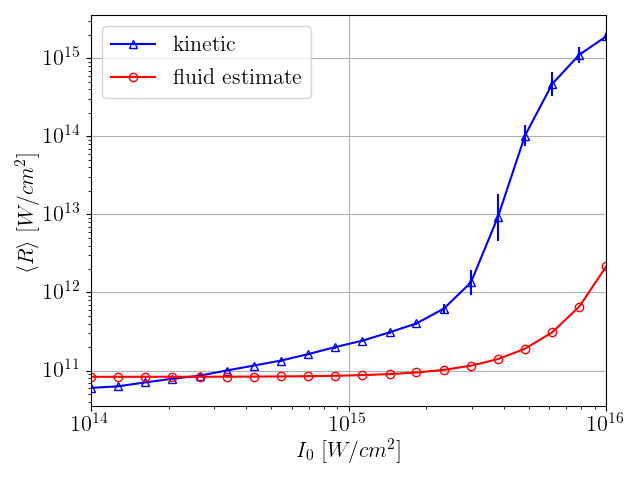
\includegraphics[width=0.99\textwidth]{Chapters/C4_iSRS/012_kinetic_fluid.png}
    \caption{Caption}
    \label{fig:0.12_inflation_threshold}
\end{figure}{}
\subsubsection{Trapping and reflectivity}
\begin{figure}
    \centering
    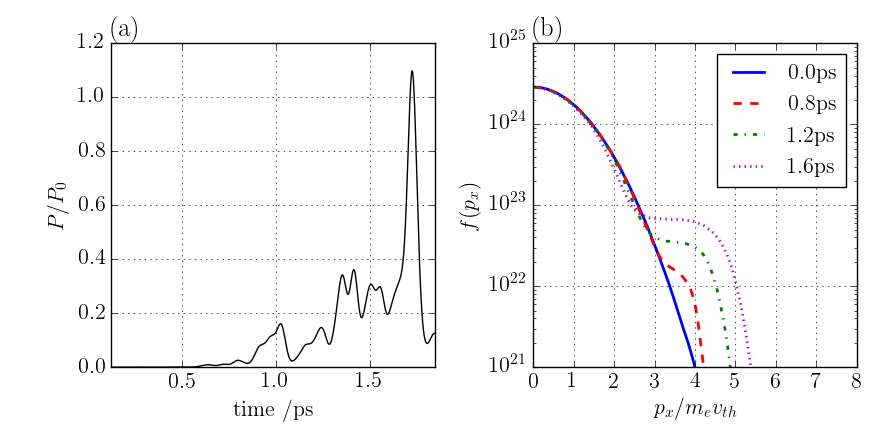
\includegraphics[width=0.99\textwidth]{Chapters/C4_iSRS/012_785e15_refl_dist.png}
    \caption{Above threshold: I = 7.85e15 Wcm-2, <R>=13.02 percent}
    \label{fig:012_refl_dist}
\end{figure}{}
\subsubsection{Freq vs X above and below threshold}
\begin{figure}
    \centering
    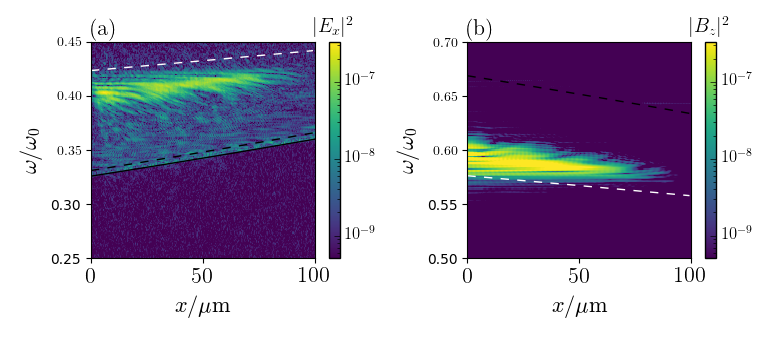
\includegraphics[width=0.99\textwidth]{Chapters/C4_iSRS/012_785e15_0_12ps_freqVsX.png}
    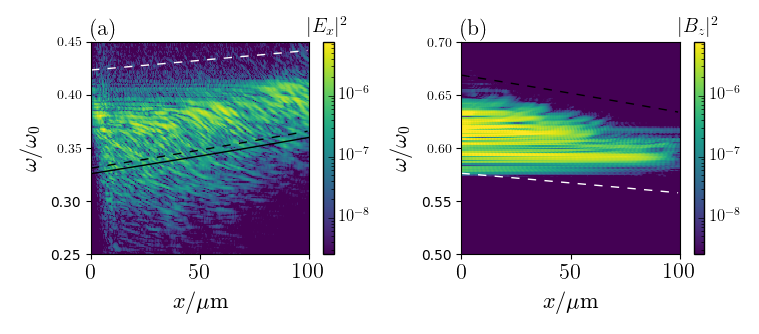
\includegraphics[width=0.99\textwidth]{Chapters/C4_iSRS/012_785e15_1_2ps_freqVsX.png}
    \caption{Above threshold: I = 7.85e15 Wcm-2, FFT between 1-2 ps and 0 - 1.2ps}
    \label{fig:012_freqVsX}
\end{figure}{}



\subsection{0.2nCrit}
\subsubsection{Inflation threshold}
\subsubsection{Trapping and reflectivity}
\subsubsection{Freq vs X above and below threshold}